\documentclass[12pt,a4]{article}




\usepackage{graphicx,amsmath,amssymb,amsthm, boxedminipage,xcolor}

%\usepackage[lined,boxed]{algorithm2e}

\usepackage{algorithm}
\usepackage{algpseudocode}

%\usepackage{algorithmic}
\usepackage{algpseudocode}
\usepackage{amsmath}
\usepackage{graphics}
\usepackage{epsfig}

\newtheorem{theorem}{Theorem}[section]
\newtheorem{proposition}[theorem]{Proposition}
\newtheorem{lemma}[theorem]{Lemma}
\newtheorem{corollary}[theorem]{Corollary}
\newtheorem{definition}[theorem]{Definition}

\newtheorem*{theorem*}{Theorem}
\newtheorem*{lemma*}{Lemma}
\newtheorem*{proposition*}{Proposition}


\newtheorem{exercise}[theorem]{Exercise}
\newtheorem{exerciseD}[theorem]{*Exercise}
\newtheorem{exerciseDD}[theorem]{**Exercise}

\let\oldexercise\exercise
\renewcommand{\exercise}{\oldexercise\normalfont}

%\let\oldexerciseD\exerciseD
%\renewcommand{\exerciseD}{\oldexerciseD\normalfont}

%\let\oldexerciseDD\exerciseDD
%\renewcommand{\exerciseDD}{\oldexerciseDD\normalfont}

\newcommand{\E}{\mathbb{E}}
%\newcommand{\nth}[1]{#1^{\textsuperscript{th}}}
\newcommand{\scalar}[2]{\ensuremath{\langle #1, #2\rangle}}
\newcommand{\floor}[1]{\left\lfloor #1 \right\rfloor}
\newcommand{\ceil}[1]{\left\lceil #1 \right\rceil}
\newcommand{\norm}[1]{\|#1\|}
\newcommand{\pfrac}[2]{\left(\frac{#1}{#2}\right)}
\newcommand{\nth}[1]{#1^{\textsuperscript{th}}}
\newcommand{\core}{\textnormal{core}}



\newif\ifsolution

\solutionfalse

\newcommand{\answer}[1]{
\ifsolution
{\color{blue} #1}
\else
\fi
}



\newcommand{\poly}{\textnormal{poly}}
\newcommand{\quasipol}{\textnormal{quasipol}}
\newcommand{\ssubexp}{\textnormal{stronglySubExp}}
\newcommand{\wsubexp}{\textnormal{weaklySubExp}}
\newcommand{\simplyexp}{\textnormal{E}}
\newcommand{\expo}{\textnormal{Exp}}



\newcommand{\N}{\mathbb{N}}
\newcommand{\nn}{\mathbb{N}_0^n}
\newcommand{\R}{\mathbb{R}}
\newcommand{\Z}{\mathbb{Z}}


\definecolor{darkgreen}{rgb}{0,0.6,0}


\date{}

\title{
  Mathematical Foundations \\of \\Computer Science\\
  \vspace{3mm}
{\normalsize CS 499,	Shanghai Jiaotong University,  Dominik Scheder}
}

\begin{document}

\maketitle

%\begin{quotation}
%  You are welcome to discuss the exercises in the discussion
%  forum. Please take them serious. Doing the exercises is as important
%  than watching the videos.
%
%  I intentionally included very challenging exercises and marked them
%  with one or two ``$*$''. No star means you should be able to solve
%  the exercises without big problems once you have understood
%  the material from the video lecture. One star means it requires 
%  significant additional thinking. Two stars means it is not 
%  unlikely that you will fail to solve them, even once you have understood
%  the material and thought a lot about the exercise. Don't feel bad
%  if you fail. Failure is part of learning.
%
%  This is the first time this course is online. Thus there might be mistakes
%  (typos or more serious conceptual mistakes) in the exercises. I will be 
%  grateful if you point them out to me!
%\end{quotation}





\setcounter{section}{10}

\section{Matchings and Network Flow}



\begin{itemize}
 \item Homework assignment published on Monday 2018-05-14
 \item Submit questions and first solutions by Sunday, 2018-05-20, 12:00
 \item Submit final solution by Sunday, 2018-05-27.
\end{itemize}


\subsection{Matchings}


Consider the Hamming cube $\{0,1\}^n$. We can view it as a graph $H_n$, 
where the vertex set is $\{0,1\}^n$ and two vertices $x,y$ are connected by an 
edge if $x$ and $y$ differ in exactly one coordinate.
Define the $\nth{k}$ layer to be 
$L_k := \{ x \in \{0,1\}^n \ | \ |x|_1 = k\}$, where $|x|_1$ denotes the number of $1$s 
in $x$. Note that the subgraph induced by layer $k$ and layer $k+1$ is a bipartite 
graph $H_n [ L_k \cup L_{k+1}]$. See the picture below for an illustration ($n=3, k=1$):
\begin{center}
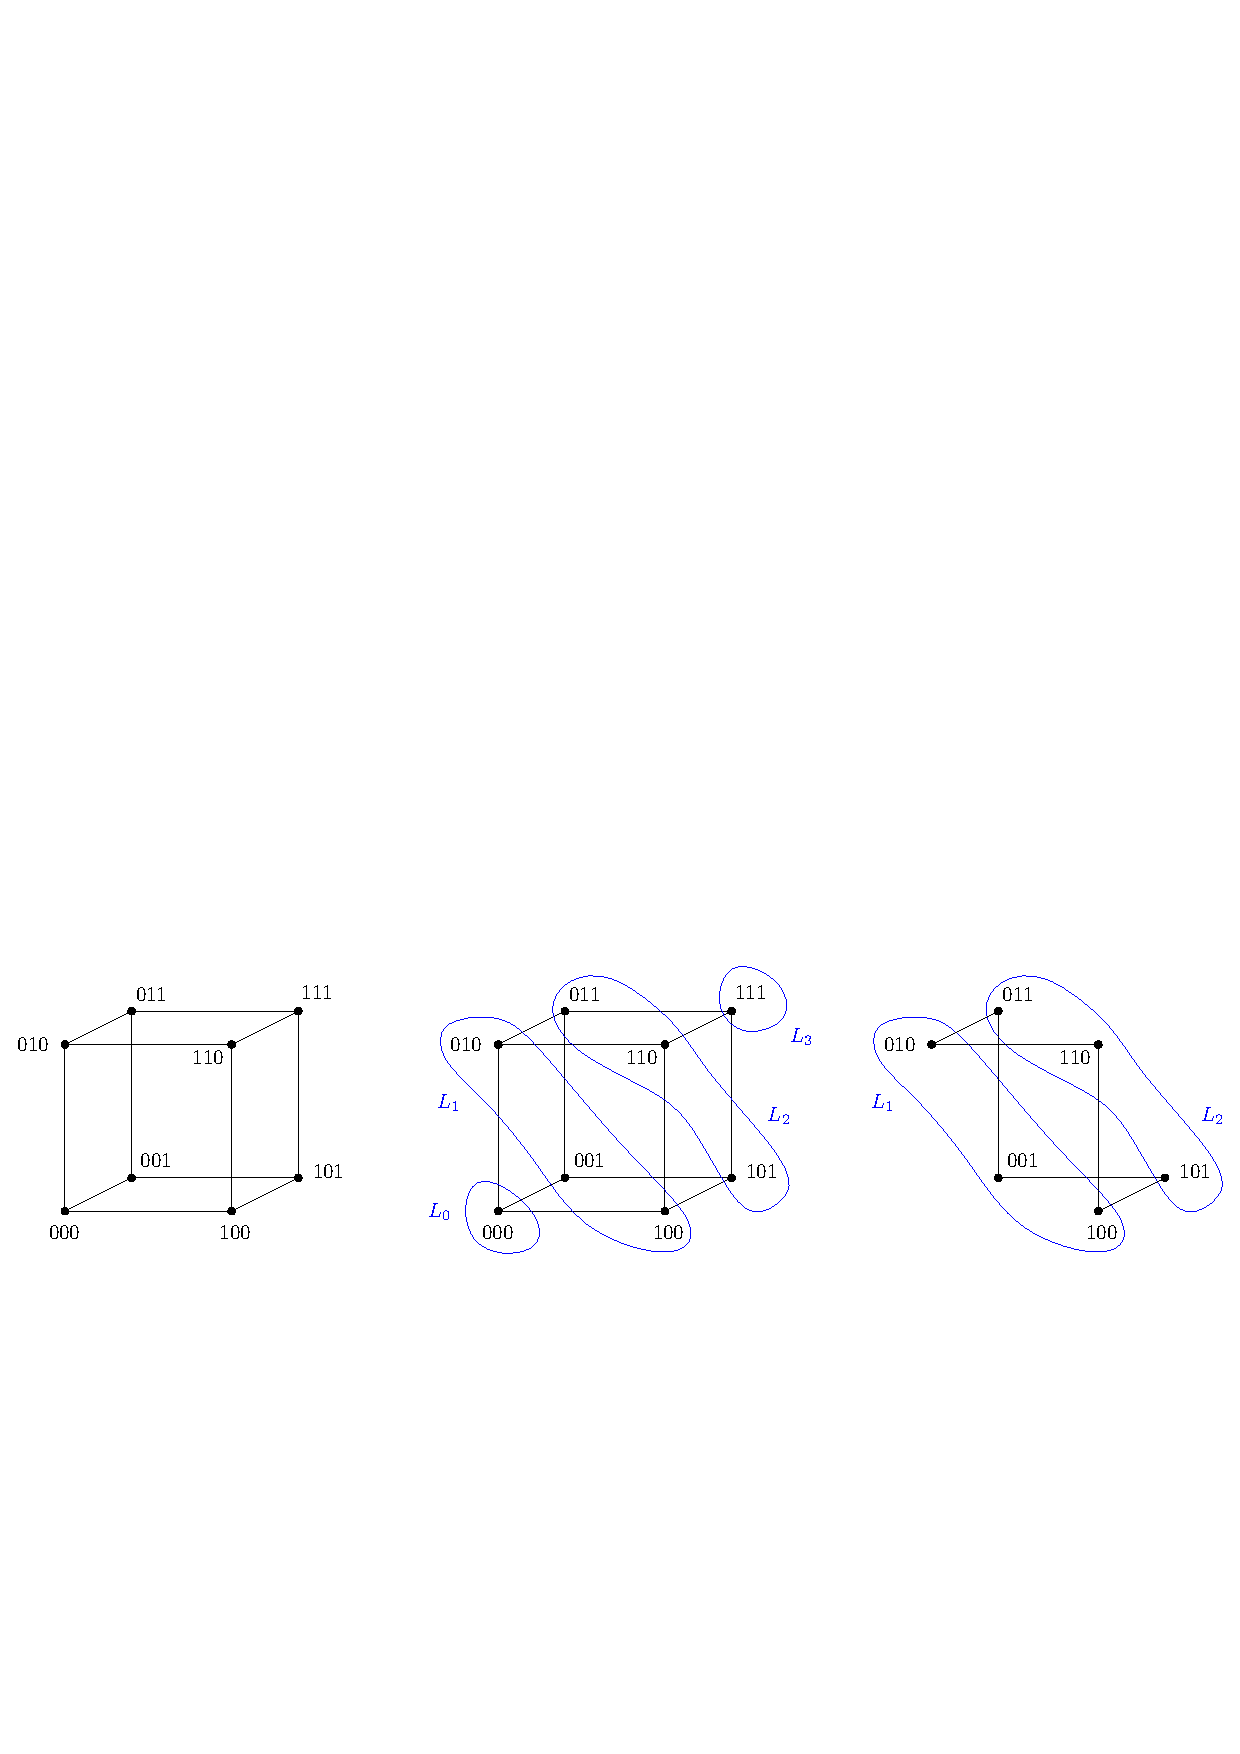
\includegraphics[width=\textwidth]{figures/hamming-cube-layer-graph.pdf}
\end{center}
\begin{exercise}
 Let $0 \leq k < n/2$.
 Show that the bipartite graph $H_n [L_k \cup L_{k+1}]$ has a matching of size $|L_k| = {n \choose k}$.
\end{exercise}

\begin{exercise}
 Let $G = (V,E)$ be a bipartite graph with left side $L$ and right side $R$.
 Suppose $G$ is $d$-regular (every vertex has degree $d$), so in particular $|L| = |R|$.
 Show that $G$ 
 has a perfect matching (that is, a matching $M$ of size $|L|$).
\end{exercise}

\begin{exercise}
  Let $G$ a $d$-regular bipartite graph. Show that the edges $E(G)$ can be partitioned
  into $d$ perfect matchings. That is, there are matchings $M_1, \dots, M_d \subseteq E(G)$ such that
  (1) $M_i \cap M_j = \emptyset$ for $1 \leq i < j \leq d$ and 
  (2) $M_1 \cup M_2 \cup \dots \cup M_d = E(G)$.
\end{exercise}

\subsection{Networks with Vertex Capacities}

Suppose we have a directed graph $G = (V,E)$ but instead of 
{\em edge capacities} we have {\em vertex capacities} $c: V \rightarrow \R$.
Now a flow $f$ should observe the {\em vertex capacity constraints}, i.e.,
the outflow from a vertex $u$ should not exceed $c(u)$:
\begin{align*}
  \forall u \in V: \sum_{v \in V, f(u,v) > 0} f(u,v) \leq c(u) \ .
\end{align*}

\begin{exercise} Consider networks with vertex capacities.
  \begin{enumerate}
    \item Show how to model networks with vertex capacities by 
      networks with edge capacities. More precisely, 
      show how to transform $G = (V,E,c)$ with $c: V \rightarrow \R^+$
      into a network $G' = (V',E',c')$ with $c': E' \rightarrow \R^+$
      such that every $s$-$t$-flow $f$ in $G$ that respects the vertex capacities 
      corresponds to an $s$-$t$-flow $f'$ (of same value) in $G'$ that
      respects edge capacities, and vice versa.
    \item Draw a picture illustrating your solution.
    \item Show that there is a polynomial time algorithm solving the
      following problem: Given a directed graph $G = (V,E)$ and two
      vertices $s,t \in V$.  Are there $k$ paths $p_1,\dots,p_k$, each
      from $s$ to $t$, such that the paths are {\em internally vertex
        disjoint}?  Here, internally vertex disjoint means that for $i
      \ne j$ the paths $p_i,p_j$ share no vertices besides $s$ and
      $t$.
  \end{enumerate}
\end{exercise}

\begin{exercise} 
  Let $H_n$ be the $n$-dimensional Hamming cube. For $i < n/2$ consider
  $L_i$ and $L_{n-i}$. Note that 
  $|L_i| = {n \choose i} = { n \choose n-i}  = L_{n-i}$, so the 
  $L_i$ and $L_{n-i}$ have the same size.   Show that there are ${n \choose i}$ paths $p_1,p_2,\dots,p_{ {n \choose i}}$
  in $H_n$ such that
  (i) each path $p$ starts in $L_i$ and ends in $L_{n-i}$;
  (ii) two different paths $p,p'$ do not share any vertices.
\end{exercise}


\subsection{Always, Sometimes, or Never Full}


Let $(G,s,t,c)$ be a flow network, $G = (V,E)$. A directed edge $e=(u,v)$ is called always full if $f(e) = c(e)$ for every maximum flow; it is called sometimes full if $f(e) = c(e)$ for some but not all maximum flows; it is called never full if $f(e) < c(e)$ for all maximum flows.

Let $(S, V\setminus S)$ be a cut. That is, $s \in S, t \in V \setminus S$. We say the edge $e = (u,v)$ is crossing the cut if $u \in S$ and $v \in V \setminus S$. We say $e$ is always crossing if it crosses every minimum cut; sometimes crossing if it crosses some, but not all minimum cuts; never crossing if it crosses no minimum cut. For example, look at this flow network:
\begin{center}
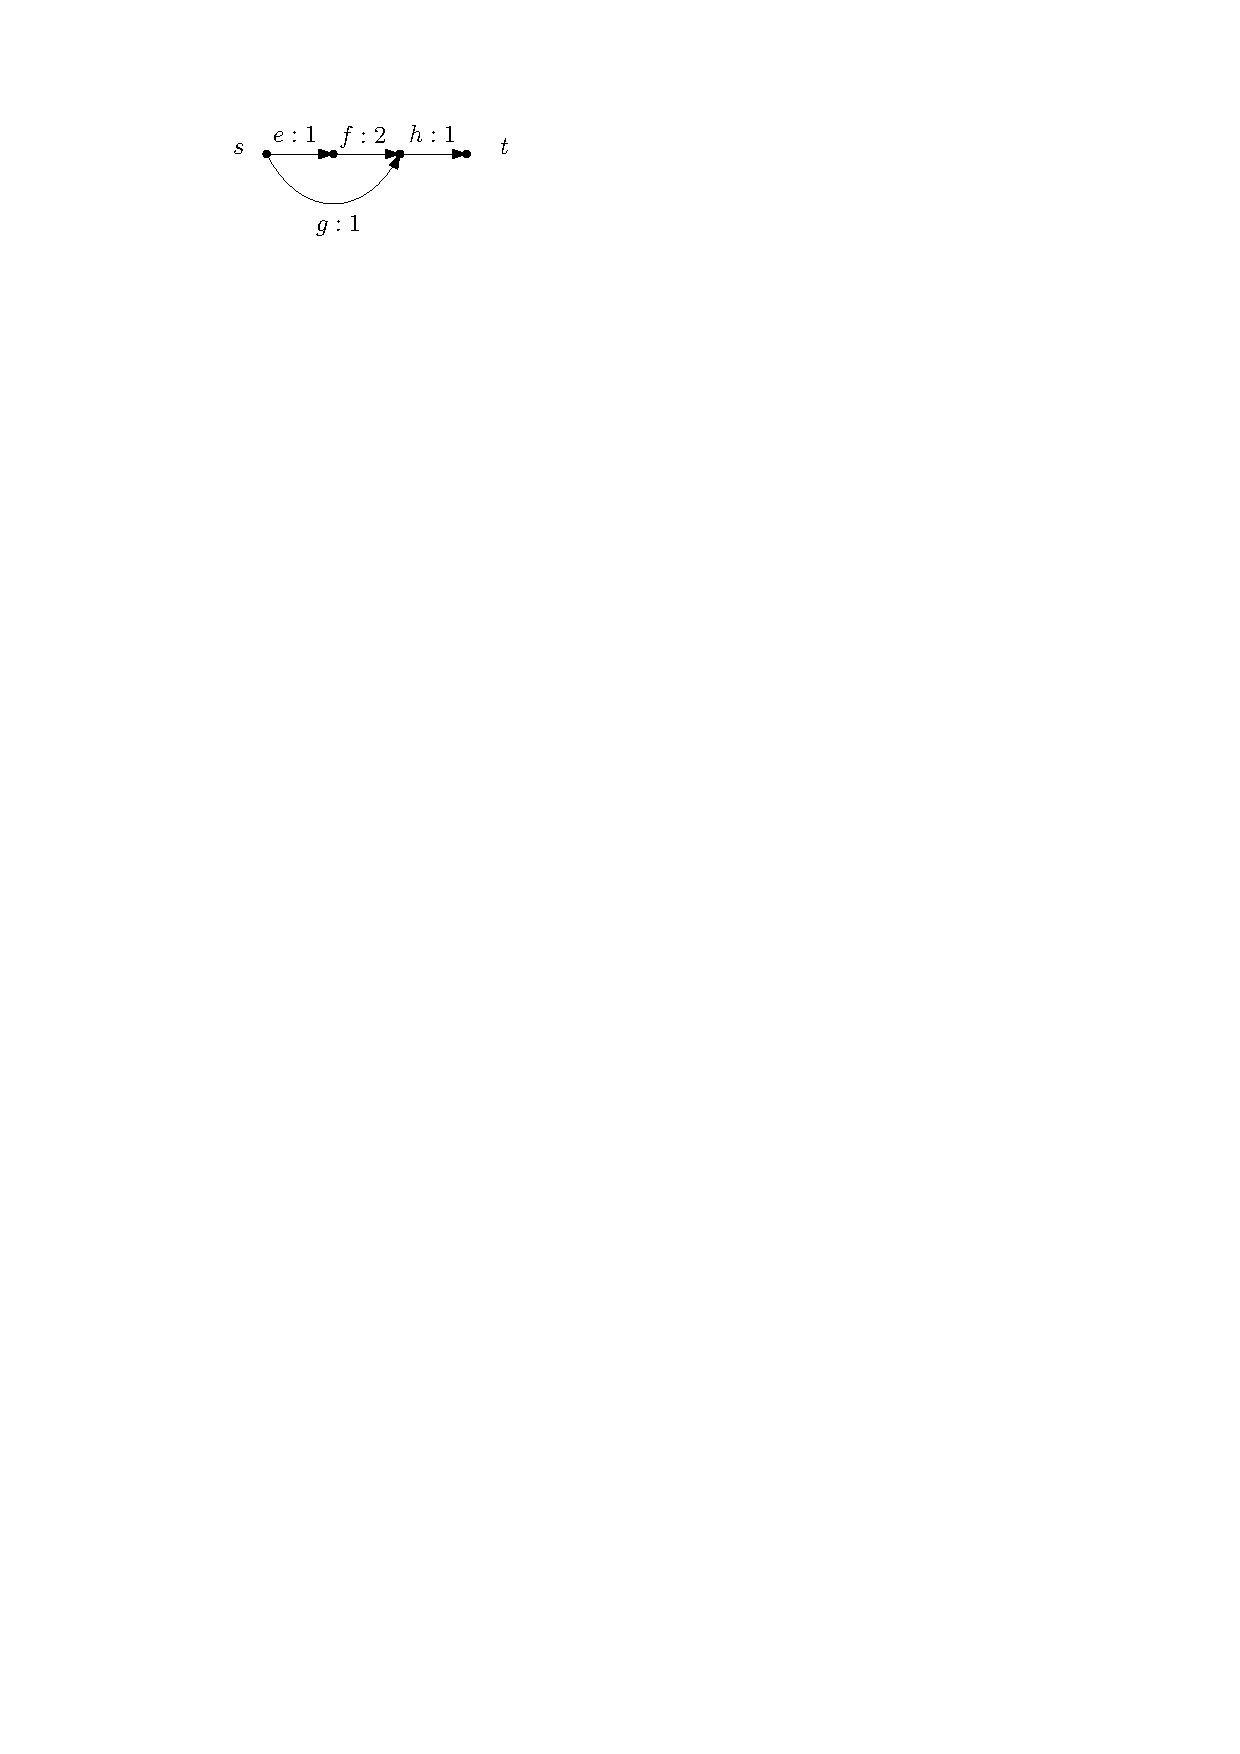
\includegraphics[width=0.4\textwidth]{figures/flow-network-always-sometimes-never.pdf}\\
\small Example network: the edges $e,g$ are sometimes full and never crossing; $f$ is never full and never crossing; $h$ is always full and always crossing.
\end{center}

\begin{exercise}
Consider this network: 
\begin{center}
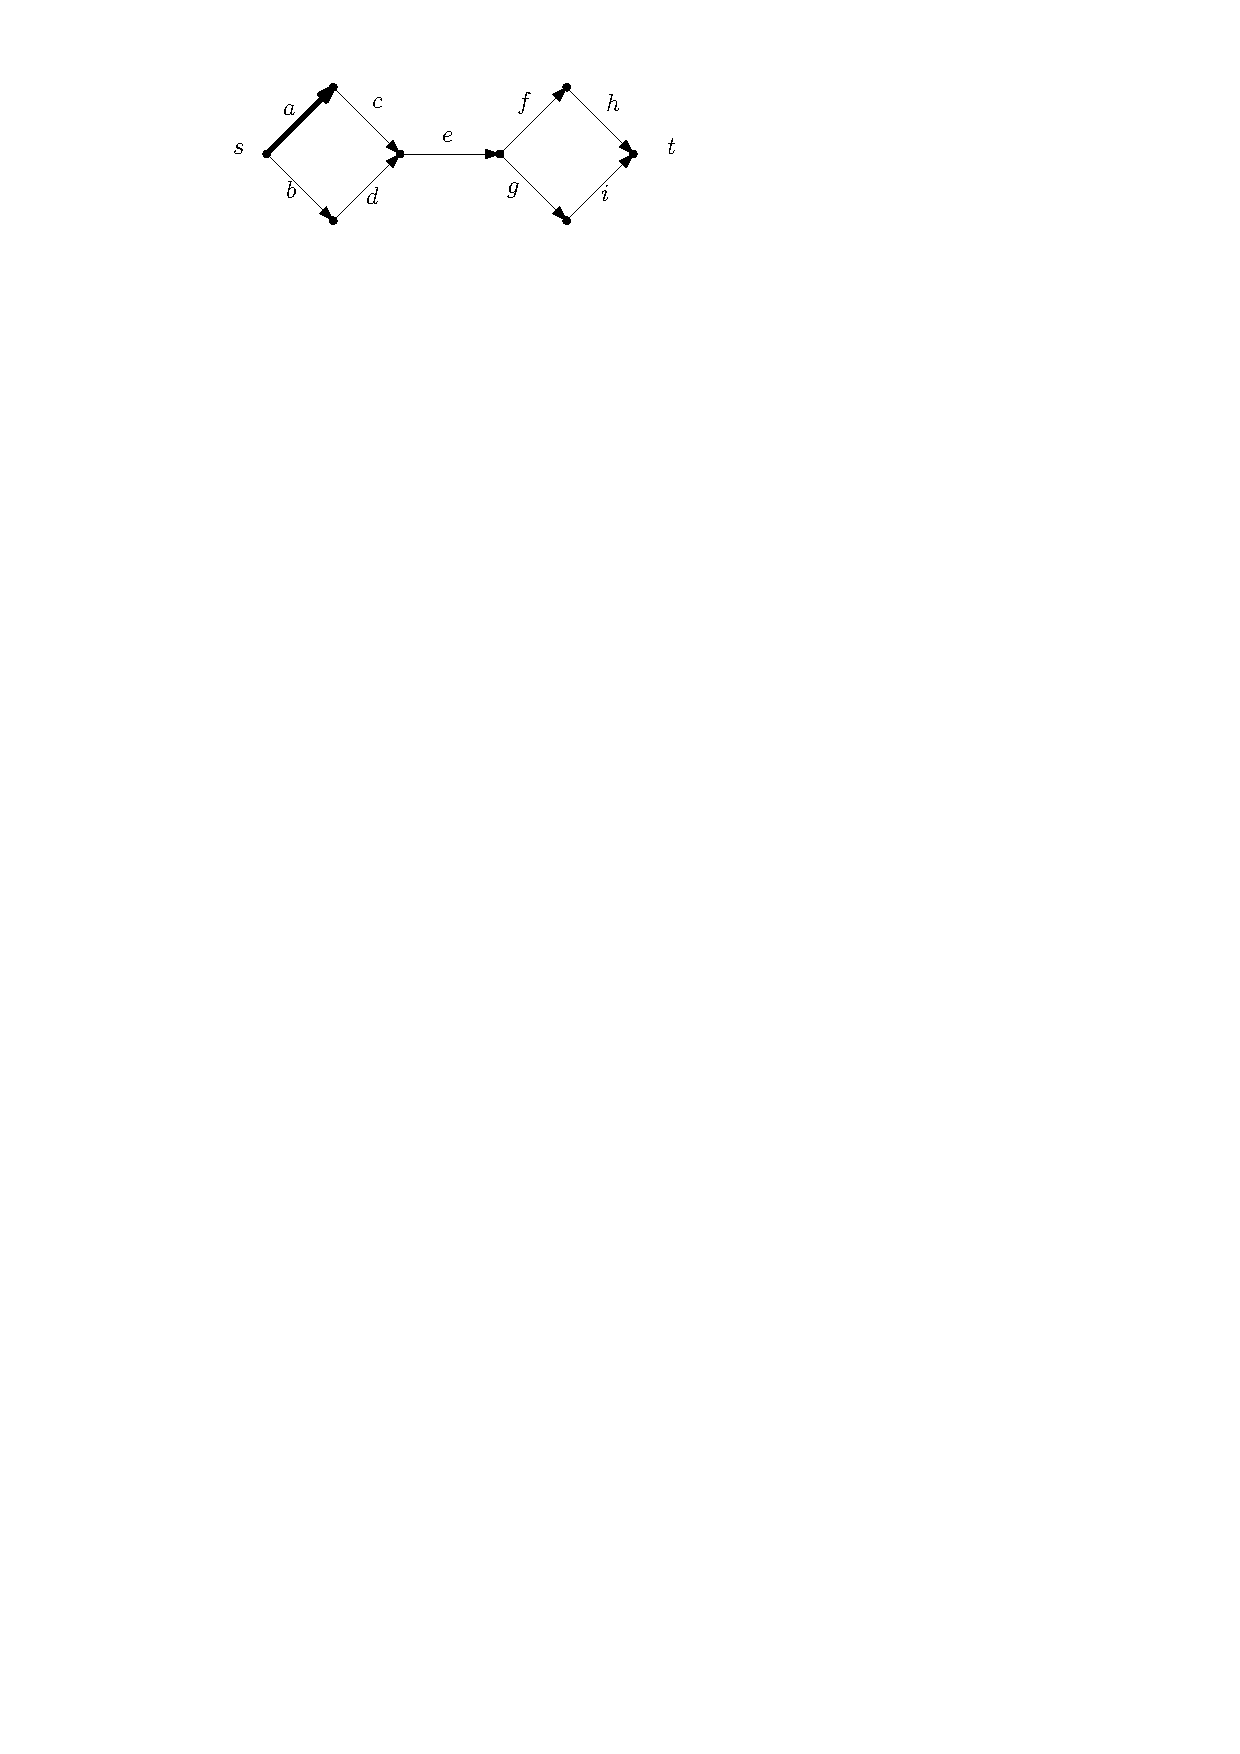
\includegraphics[width=0.6\textwidth]{figures/other-flow-network-always-sometimes-never.pdf}\\
\small The fat edge $a$ has capcity $2$, all other edges have capacity $1$.
\end{center}
\begin{enumerate}
\item Indicate which edges are (i) always full, (ii) sometimes full, (iii) never full.
\item Indicate which edges are (i) always crossing, (ii) sometimes crossing, (iii) never crossing.
\end{enumerate}
\end{exercise}

\begin{exercise}
An edge $e$ can be ($x$) always full, ($y$) sometimes full, ($z$) never full; it can be ($x$') always crossing, ($y'$) sometimes crossing, ($z'$) never crossing. So there are nine possible combinations: ($xx'$) always full and always crossing, ($xy'$) always full and sometimes crossing, and so on. Or are there? Maybe some possibilities are impossible. 
Let's draw a table:
\begin{center}
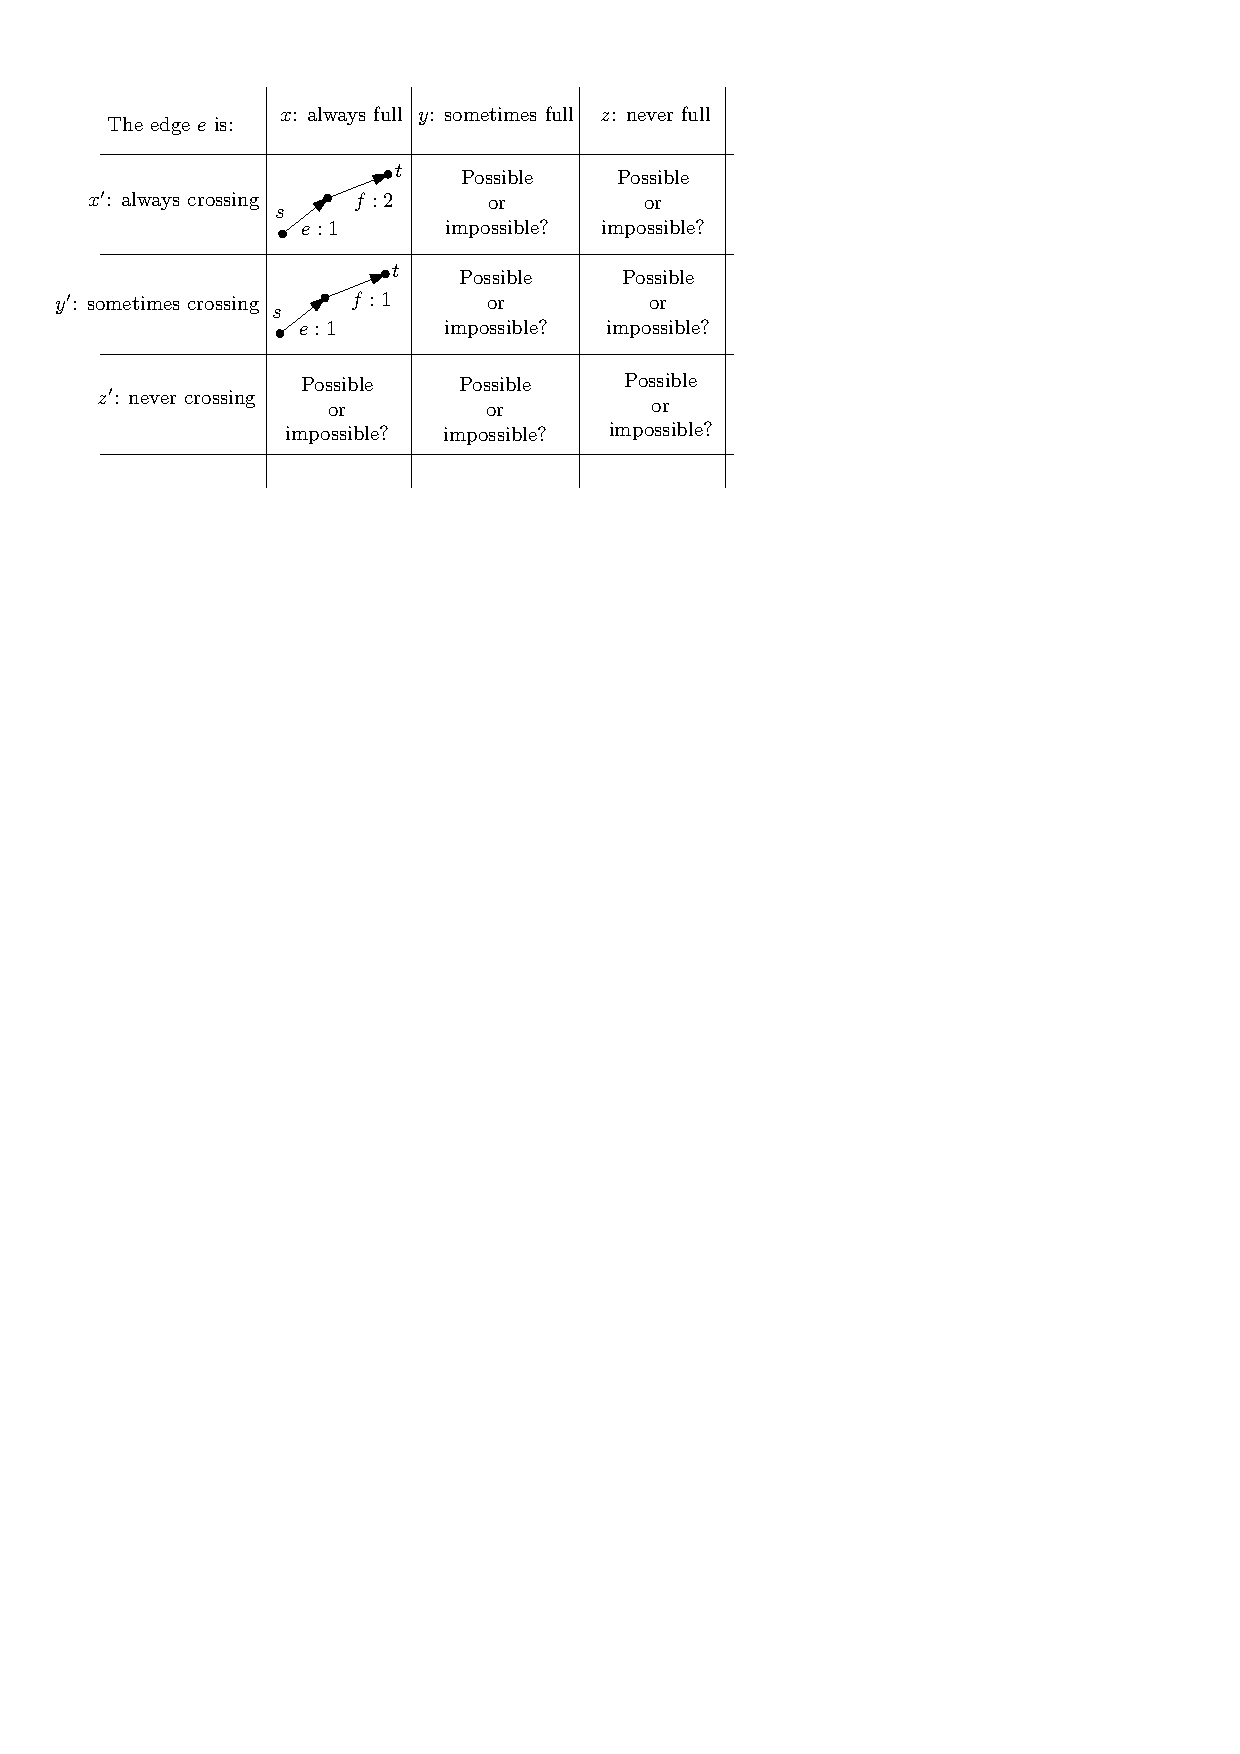
\includegraphics[width=0.8\textwidth]{figures/always-somtimes-never-table.pdf} \\
\small The nine possible cases, some of which are maybe impossible.
\end{center}
The two very simple flow networks in the table already show that $(xx')$ and $(yy')$ are possible; that is,
it is possible to be always full and always crossing, and it is possible to be always full and sometimes crossing.
Fill out the table! That is, for each of the remaining seven cases, find out whether it is possible or not. If it is
possible, draw a (simple) network showing that it is possible; if impossible, give a proof of this fact.
\end{exercise}

\end{document}
